\documentclass[12pt]{report}
\usepackage{xcolor} % for different colour comments
\usepackage{parskip} % Space between each paragraph.
%\usepackage{hardwrap} % for text length of 80 pts
\usepackage[margin=1.2in]{geometry}
\usepackage{hyperref}
\usepackage{../ltx/edcomms}
\usepackage{graphicx}
\usepackage[section]{placeins} % Prevents floats from floating across sections
\usepackage{natbib}%Bibtex
\usepackage{float}
\usepackage{tabularx}
\usepackage{ltablex} %% Multi page tables 
\usepackage{booktabs}
\usepackage{tabto}
\usepackage{tocloft} %% This package prevents table of contents from generating a page break
\usepackage{caption}
\usepackage{listings}
\usepackage{ifthen}
\usepackage{../ltx/edcomms}

%% Comments are enabled and disabled by 'draft' mode. I hacked in my own draft
%% mode (https://en.wikibooks.org/wiki/LaTeX/Macros) because the LaTeX draft
%% mode disables a bunch of things that I don't want it to. I just want it to
%% disable comments. Do not set any of this manually, just use the build script,
%% which builds both draft and final copies. Comments are enabled by default, so
%% if you build manually, you get a draft copy. 
\providecommand\draftmode{true}

\ifthenelse{\equal{\draftmode}{true}}{
\newcommand{\authornote}[3]{\textcolor{#1}{[#3 ---#2]}}
\newcommand{\todo}[1]{\textcolor{red}{[TODO: #1]}}
%\edcommstrue %% Dr. Kahl's comment package. Eventually we should migrate all
             %% comments to this.
}{
\edcommsfalse 
\newcommand{\authornote}[3]{}
\newcommand{\todo}[1]{}
}

% wss = Dr. Smith ; ds = Dr. Szymczak
\newcommand{\wss}[1]{\authornote{magenta}{SS}{#1}}
\newcommand{\ds}[1]{\authornote{blue}{DS}{#1}}


\usepackage{geometry}
\usepackage{changepage}
\usepackage{amsbsy}
\usepackage{amssymb}
\usepackage{fancyvrb}
\usepackage{listings}
\usepackage[fleqn]{amsmath}
\usepackage{graphicx}
\graphicspath{ {../figures/} }
\setlength{\parindent}{15pt} % parskip sets this to 0. 15 is default.

\newcolumntype{C}[1]{>{\centering}p{#1}} %% For use with tabularx
%%%%%%%%%%%%%%%	START OF DOCUMENT %%%%%%%%%%%%%%%%%%%%
\edcommsfalse
\begin{document}

\pagenumbering{roman} %% Roman numerals before actual document starts
\begin{titlepage}\begin{center}
\thispagestyle{empty} %% No page no. on title

\vspace*{1cm}

{\Huge\textbf{Ampersand Event-Condition-Action Rules}}

\vspace{0.5cm}
{\Large Test Plan

\vspace{1.5cm}
Yuriy Toporovskyy,\ Yash Sapra,\ Jaeden Guo}
\vfill 
%% 

%% We acknowledge that this document uses material from the Volere Requirements
%% Specification Template, copyright 1995 - 2012 the Atlantic Systems Guild
%% Limited.

%% \vspace{0.8cm}
\end{center}
CS 4ZP6 \\
October 30th, 2015 \\ 
Fall 2015 / Winter 2016 
\end{titlepage}

%% Revision history

\begin{table}[ht!]\begin{center}
\caption{Revision History}  
\begin{tabular}{|l|l|l|}\hline
\textbf{Author} & \textbf{Date} & \textbf{Comment} \\\hline 
Yuriy Toporovskyy & 03 / 11 / 2015 & Version 0 \\\hline
Yuriy Toporovskyy & 27 / 10 / 2015 & Reorganized document \\\hline
Yuriy Toporovskyy & 27 / 10 / 2015 & Initial version - template \\\hline
\end{tabular}
\end{center}\end{table}

\newpage

\tableofcontents
%% \listoffigures 
%% \listoftables 

\newpage
\pagenumbering{arabic} %% Arabic numerals in actual document

%%%%%%%%%%%%%%%%%%%%%%%%
%
%	1.) General Information 
%
%%%%%%%%%%%%%%%%%%%%%%%%

\chapter{General Information}\label{ch:General}

%1.1 Purpose/Summary
\section{Purpose}\label{sec:Purpose}
This document outlines the test plan for ECA for Ampersand, including our
general approach to testing, system test cases, and a specification of
methodology and constraints. This test plan is centered around our contribution 
to Ampersand and ignores other elements of the Ampersand process such as the 
artifacts that are generated.

%% %1.3 Objectives
\section{Objectives}\label{sec:Objectives}
\subsubsection*{Preparation for testing}
The primary objective of this test plan is to gather all relevant information 
that could aid in creating effective tests for EFA. EFA in this regard is 
modularized and tested as an individual component before it is tested within 
the Ampersand system. 

\subsubsection*{Communication}
This test plan intends to clearly communicate to all developers of ECA for 
Ampersand their intended role in the testing process. 

\subsubsection*{Motivation}
The testing approach is based on the constraints and requirements presented in 
the Software Requirements Specification \big( i.e. SRS\big). This document 
focuses on 
how the functional and non-functional requirements provided in the SRS will be 
tested for this project.

\subsubsection*{Environment}
This test plan outlines the resources, tools, and software required for the
testing process. This includes any resources needed to perform automated testing. 

\subsubsection*{Scope}
This test plan intends to better describe the scope of our contribution, ECA,
within the Ampersand system. 

%% %1.3  Definitions, Acronyms, and abbreviations 
\section{Definitions}\label{sec:Abbrev}

\subsubsection*{SRS}
Software Requirements Specification. Document regarding requirements, constraints, and project objectives.

\subsubsection*{EBNF}
Extended Backus–Naur Form. A notation for specifying the syntax of languages, see \cite{ebnf}.

\subsubsection*{RA}
Relation algebra. The mathematical language used in ADL files to specify business rules. 

\subsubsection*{PA}
Process algebra. The mathematical language used by ECA rules to describe the
action to be taken to fix violations. A ``PA clause'' (also written as
``PAclause''), or process algebra clause, is an imperative-style language which
represents the \emph{mathematical} process which Ampersand uses. The syntax of
PA clauses, in EBNF notation, is as follows: \edcomm{JG}{What is EBNF?}
%% YT: this is a subset of the actual language... I don't actually understand the rest

\begin{lstlisting}[basicstyle=\ttfamily]
PAclause ::= 'One' '(' PAclause { ',' PAclause } ')' ; 
           | 'Choice' '(' GPAclause { ',' GPAclause } ')' ;  
           | 'All' '(' PAclause { ',' PAclause } ')' ;  
           | ('Ins' | 'Del') '(' RExpr ',' RAtom ')' ; 
           | 'Nop'  
           | 'Blk' 
GPAclause ::= RExpr '->' PAclause ; 
\end{lstlisting}
where ``RExpr'' represents RA expressions, and ``RAtom'' (RA atom) represents
\emph{atomic} RA expressions (i.e. terms with no operators).

\begin{table}[ht!]\begin{center}\label{tab:PASemantics}
\caption{Semantics of PAclause terminals}
\begin{tabularx}{\textwidth}{lX}
One$(p_0 \ldots p_n)$ & Execute exactly one of $p_0 \ldots p_n$. \\
Choice$(g_0 \rightarrow p_0 \ldots g_n \rightarrow p_n)$ & Execute exactly
  one of $p_i$, such that $g_i$ is a non-empty RA term. \\
All$(p_0 \ldots p_n)$ & Execute all of $p_0 \ldots p_n$. \\
$<$Ins/Del$>(e,r)$ & Insert or delete the expression $e$ from the relation $r$. \\
Nop & Do nothing. \\
Blk & The null command, which blocks forever. 
\end{tabularx}
\end{center}\end{table}

The semantics of process algebra says that the ``choice'' operators (e.g. One
and Choice) may execute any one of their subclauses; if \emph{any} of the
subclauses can be completed, the PA clause has restored the violation.  One
choice may be considered better in some ways, for example, different
alternatives could have vastly different execution costs. For the purpose of
this document, however, we will make the simplest ``choice'' possible, which
generally means an arbitrary choice. 

\subsubsection*{ECA Rule}
 Event-Condition-Action Rule. A rule which describes how to handle a constraint
 violation in a database. The syntax of ECA rules is as follows:

\begin{lstlisting}[basicstyle=\ttfamily]
ECArule ::= 'On' ('Ins' | 'Del') 
            '(' RExpr ',' RAtom ')'
            'Do' PAclause    
\end{lstlisting}

\subsubsection*{HUnit}
 A Haskell library for unit testing. See section \ref{sec:TestTools}.
\subsubsection*{QuickCheck}
 A Haskell library for running automated, randomized tests. See section 
 \ref{sec:TestTools}.
 
 \subsubsection*{Sentinel}
A test server accessible through the Ampersand webcite (\cite{sentinellink}) which executes a set of 
randomly generated tests on Ampersand on a daily basis, see \cite{sentinel} for details.

%%%%%%%%%%%%%%%%%%%%%%%%
%
%	2.) Plan
%
%%%%%%%%%%%%%%%%%%%%%%%%

\chapter{Plan}\label{ch:Plan}

\section{Software Description}\label{sec:SoftwareDesc}
Ampersand is a software tool that converts the formal specifications of 
business entities and rules, compiles it into various design artifacts (e.g. 
latex documents), and produces a prototype web application.

The business prototype implements business logic according to specifications 
provided by the user, it uses the entities and relationships that the user 
provides to form a relational database with a simple web application front-end.

ECA for Ampersand focuses on automatically restoring a particular class of 
database violations using an algorithm called AMMBR \cite{amber}.  This class 
of violations is realized within Ampersand as ECA rules -- our contribution to 
Ampersand will add support for ECA rules, that will affect Ampersand's back-end 
as well as the generated prototype it provides.

\edcomm{YT}{Probably should merge Test Team and Test Schedule}
\section{Test Team}\label{sec:TestTeam} \edcomm{JG}{You did a great job! could 
you explain to me what a test schedule is?}

The test team which will execute the strategy outline in this document is comprised of
\begin{itemize}
\item Yuriy Toporovskyy  
\item Yash Sapra        
\item Jaeden Guo         
\end{itemize}

\section{Test Schedule}\label{sec:TestSched}
\begin{center}
 	\begin{tabular}{| c | c| } \hline
 		Dates & Tests to be performed \\ \hline
 		12-20-2015 - 01-07-2016 & Unit testing, black box testing, \\ & white 
 		box 
 		testing with heavy use \\ & of QuickCheck  \\ \hline
 		01-08-2016 - 01-20-2016 & System testing EFA with Ampersand  \\  \hline
 	 01-20-2016-02-01-2016     & Testing for abnormality and performance. \\ 
 	 \hline     
 	\end{tabular}
 \end{center}|

 \emph{Note:} More details for specific test will be provided in the future.
\chapter{Methods and constraints}\label{ch:Methods}
\section{Methodology}\label{sec:Methodology}
A Waterfall Development methodology is used in combination with Software 
Prototyping and will likely result in something similar to the spiral model. 
The Waterfall method help translate the requirements outlines in the SRS into 
functional and non-functional requirements that the design must include. 
Furthermore, as Software Prototyping is not a standalone method, but rather an 
approach to development activities these two compliment each other well.
\begin{center}
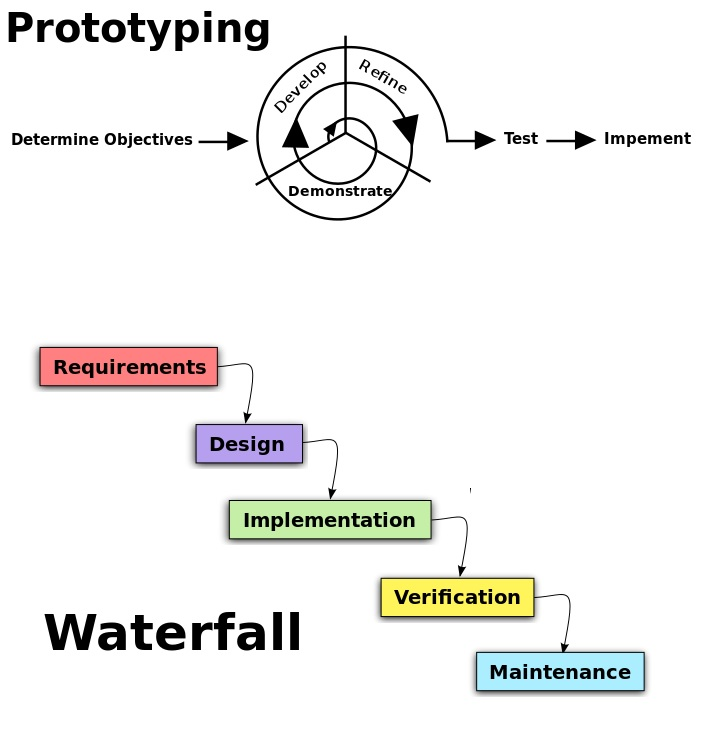
\includegraphics[scale=0.5]{testing}
\end{center}|
\section{Test tools}\label{sec:TestTools}

Various tools are used by the existing Ampersand developers to test
Ampersand. In order to integrate best with Ampersand, our code will adopt their
test tools. 

%% This doesn't make grammatical sense?
%% See section \ref{subsec:RandTest} for QuickCheck.

%% In addition to QuickCheck, Sentinel Test will be used for the completed 
%% Ampersand system test. Since EFA will be incorporated into Ampersand, it must 
%% pass all sets of randomly generated tests. 

\subsection{Static Typing}\label{subsec:Static}
Programming languages can be classified by many criteria, one of which is their
type systems. One such classification is static versus dynamic typing. Our
implementation language, Haskell, has a static type system. Types will be
checked at compile-time, allow us to catch errors even before the code is run,
reducing the errors that need to be found and fixed using testing techniques. 

\edcomm{YT}{``Static analysis'' is the analysis of a program without running it,
  ie, analysis of the program text. We won't be doing any static analysis, I
  believe... QuickCheck is absolutely unrelated to static analysis.}
\subsection{Formal verification}\label{subsec:FormalVer}
A part of our project deals with generating source code annotated with the proof
of derivation of that source code, which will act as a correctness proof for the
system. In particular, when we generate code to restore a database violation
using ECA rules, then the generated code will have a RA proof associated with it,
which details how that code was derived from the original specification given by
the user.

\subsection{Random Testing}\label{subsec:RandTest}
Random testing allows us to easily run a very large number of tests without
writing them by hand, and also has the advantage of not producing biased test
cases, like a programmer is likely to do.

We will be using QuickCheck \cite{hackage} for random testing. The existing 
Ampersand code base
using QuickCheck for testing, therefore, using QuickCheck has the added benefit
of easier integration with the existing Ampersand code base.

QuickCheck allows the programmers to provide a specification of the program, in
the form of properties. A property is essentially a boolean valued Haskell
function of any number of arguments. QuickCheck can test that these properties
hold in a large number of randomly generated cases. QuickCheck also takes great
care to produce a large variety of test cases, and generally produces good code
coverage. QuickCheck will be used for individualized module testing and well as 
provide a fair array of random tests for the combination of all modules 
\cite{hackage}.

\edcomm{YT}{Don't assume that this super obvious example will make sense... better to leave it out.}

%% \begin{lstlisting}
%% quickCheck (\s -> length (take5 s) == 5)
%% Falsifiable, after 0 tests:
%% ""
%% \end{lstlisting}

%% Here we test that the length of a list after implementing ``take 5'' should be 5 however this fails when the initial list is empty or has less than 5 elements.
\subsection{Unit Testing}\label{subsec:UnitTest}
Unit testing is comprised of feeding some data to the functions being tested and
compare the actual results returned to the expected results.
We will be using HUnit for unit testing of the new source code 
\edcomm{YT}{HUnit does not do *automated* testing.}in Ampersand. HUnit is a 
library providing unit testing capabilities in Haskell.  It is an adaption of 
JUnit to Haskell that allows you to easily create, name, group tests, and 
execute them.

\section{Requirements}\label{sec:Reqs}
Requirements are the main motivator for tests and test methodoloy -- testing
should help ensure that requirements are met. To this end, our requirements are
briefly summarized and labelled below.

\subsection{Functional requirements}\label{subsec:FunReqs}
The functional requirements for ECA for Ampersand are detailed in the SRS; they
are also briefly summarized here. Our implementation must

\begin{description}
\item[F1] provably implement the desired algorithm.
\item[F2] accept its input in the existing ECArule format.
\item[F3] produce an output compatible with the existing pipeline. 
\item[F4] annotated generated code with proofs of correctness or derivations,
where appropriate. 
\item[F5] automatically fix database violations in the mock database of the
prototype.
\item[F6] not introduce appreciable performance degradation. 
\item[F7] provide diagnostic information about the algorithm to
the user, if the user asks for such information.
\end{description}

\subsection{Non-Functional requirements}\label{subsec:NonFunReqs}
The functional requirements for ECA for Ampersand are detailed in the SRS; they
are also briefly summarized here. Our implementation must

\begin{description}
\item[N1] produce output which will be easily understood by the typical user,
  such as a requirements engineer, and will not be misleading or confusing.  
\item[N2] be composed of easily maintainable, well documented code.
\item[N3] compile and run in the environment currently used to develop
  Ampersand.
\item[N4] be a pure function; it should not have side effects.  
\end{description}

\section{Data recording}\label{sec:DataRec}
Not Available at this time.
\section{Constraints}\label{sec:Constraints}
Not applicable at this time.
%% \section{Evaluation}\label{sec:Evaluation}
%% Due to the early stage of development, this is not available at this time.
%%%%%%%%%%%%%%%%%%%%%%%%%
%%
%%	5.) System Test Description
%%
%%%%%%%%%%%%%%%%%%%%%%%%%

\chapter{System Test Descriptions}\label{ch:SystemTests}
\newcommand{\us}{\textunderscore}
\newcommand{\tabb}{\hspace{35pt}}
%% Environment for system test
\newcounter{sysTestNum}
\setcounter{sysTestNum}{1}

%% Commands for making ECA rules in math environments 
\newcommand{\ECAIns}[2]{\mathbf{Ins}(#1,#2)}
\newcommand{\ECADel}[2]{\mathbf{Del}(#1,#2)}
\newcommand{\ECAInsDel}[2]{\mathbf{\{Ins/Del\}}(#1,#2)}
\newcommand{\ECADelIns}[2]{\mathbf{\{Del/Ins\}}(#1,#2)}
\newcommand{\ECAOn}{\mathbf{On~}}
\newcommand{\ECADo}{\ECASpacer\mathbf{Do~}}
\newcommand{\ECANop}{\mathbf{Nop~}}
\newcommand{\ECASpacer}{\,\,\,\,}
\newcommand{\IRel}[1]{\mathbb{I}_{#1}}
\newcommand{\VRel}[2]{\mathbb{V}_{#1\times#2}}

\newcommand{\systemTest}[5]{
\section*{T\arabic{sysTestNum}~~~ #2}\label{sec:#1}
\addcontentsline{toc}{section}{T\arabic{sysTestNum}~~~ #2}
\stepcounter{sysTestNum}
\hspace{-6pt}\begin{tabular}{p{3cm}l}
\textbf{Test type}     &   #3 \\ 
\textbf{Schedule}      &   #4 \\
\textbf{Requirements}  &   #5 \\
\end{tabular}
}


Many test cases use domain specific language to indicate inputs and outputs, for
both clarity and brevity. This includes the syntax and semantics of ECA rules
and Abstract SQL. For the full syntax and semantics of these, as well as
related definitions, see section \ref{sec:Abbrev}.

%% %% Example usage....
%% \systemTest{T1}  %% Test label, should be unique
%% {EFA Black box test}  %% Test name
%% {Black box/Functional, using dynamic analysis}  
%% {January 2016 }
%% {Functional}

%% The input shall consist of PAClauses (i.e. a data type) that is composed of 
%% ECA rules. These ECA rules consist of a condition (i.e. ecaTriggr) that 
%% initiates a set of actions to be taken (i.e. ecaAction) based on the violation 
%% (i.e. ecaDelta). Please see example below for further elaboration.

%% The functional output shall be a SQL command template generated through a 
%% Haskell script, for each type of ECA violations

%% QuickCheck  is used to test the functionality of individual functions; it is a 
%% package that provides a library for testing program properties. The programmer 
%% is able to provide properties they want tested in their program specification, 
%% and QuickCheck generates numerous random cases to test that the property 
%% holds\cite{hackage}. 

%% \edcomm{JG}{So.. I originally put the entire example 
%% in Procedure and latex got very mad at me... so if you wanna put all that in 
%% here, 
%% feel free too or add/give a brief description (or I will) for those that do not 
%% want an example cause they find this self-explanatory =) 

%% Also, there are comments, but the comments can be taken out then shown for the 
%% white box test as a walk through sorta thing, am I making sense?}


%%%%%%%%%%%%%%%%% Test 1 
\systemTest{ecaInsIntoAll}
{ECA rule executing ``All'' subclauses}  %% Test name
{Dynamic, black box, automated}  
{Term 2}
{F1}
\vspace{-12pt}\subsubsection*{Input}
The input is an ECA rule of the form:

$\ECAOn \ECAIns{\Delta}{r_0} \ECADo \mathbf{All} ( \ECAIns{e_1}{r_1}, \ECAIns{e_2}{r_2} )$
\vspace{-10pt}\[\hspace{-20pt}\begin{array}{lll}
\text{where} & r_0, r_1, r_2    & := \text{Atomic Relation} \\ 
             & e_1, e_2, \Delta & := \text{Expression} \\ 
\end{array}\]

\vspace{-12pt}\subsubsection*{Output}

The output is an abstract SQL function of the form:
\begin{verbatim}
f (delta, r_0):
  INSERT INTO <r_1_table> VALUES <e_1_query>;
  INSERT INTO <r_2_table> VALUES <e_2_query>;
\end{verbatim}

\vspace{-12pt}\subsubsection*{Description}

ECA rules of the input format are generated using QuickCheck, converted to
  abstract SQL, then compared against the expected output format using HUnit.

%%%%%%%%%%%%%%%%% Test 1 
\systemTest{ecaInsIntoChoice}
{ECA rule executing ``Choice'' subclauses}  %% Test name
{Dynamic, black box, automated}  
{Term 2}
{F1}
\vspace{-12pt}\subsubsection*{Input}
The input is an ECA rule of the form:

$\ECAOn \ECAIns{\Delta}{r_0} \ECADo \mathbf{Choice} ( p_0, p_1 )$
\vspace{-10pt}\[\hspace{-20pt}\begin{array}{lll}
\text{where} & r_0   & := \text{Atomic Relation} \\ 
             & \Delta & := \text{Expression} \\ 
             & p_0, p_1 & := \text{PA Clause} \\
\end{array}\]

\vspace{-12pt}\subsubsection*{Output}

The output is an abstract SQL function of the form:
\begin{verbatim}
f (delta, r_0):
  <p_i_statement>
\end{verbatim}
where $i \in \{ 0, 1 \}$. 

\vspace{-12pt}\subsubsection*{Description}

ECA rules of the input format are generated using QuickCheck, converted to
  abstract SQL, then compared against the expected output format using HUnit.

%%%%%%%%%%%%%%%%% Test 2
\systemTest{ecaEmptyClause}
{ECA rule with empty PA clause} 
{Dynamic, black box, automated}  
{Term 2}
{F1}
\vspace{-12pt}\subsubsection*{Input}
The input is an ECA rule of the form:

$\ECAOn \ECAInsDel{\Delta}{r_0} \ECADo \ECANop $
\vspace{-10pt}\[\hspace{-20pt}\begin{array}{lll}
\text{where} & C_0, C_1 & := \text{Concept} \\ 
             & r_0      & := \text{Atomic Relation} \\ 
\end{array}\]

\vspace{-12pt}\subsubsection*{Output}

The output is the empty abstract SQL statement; that is, a statement of the form:
\begin{verbatim}
f (delta, r_0): {} \\ Do nothing
\end{verbatim}

\vspace{-12pt}\subsubsection*{Input}

ECA rules of the input format are generated using QuickCheck, converted to
  abstract SQL, then compared against the expected output format using HUnit.


%%%%%%%%%%%%%%%%% Test 3
\systemTest{ecaIdentityRel}
{ECA rule inserting into Identity relation} 
{Dynamic, black box, automated}  
{Term 2}
{F1}
\vspace{-12pt}\subsubsection*{Input}
The input is an ECA rule of the form:

$\ECAOn \ECAInsDel{\Delta}{r_0} \ECADo \ECADelIns{e_0}{\IRel{C_0}} $
\vspace{-10pt}\[\hspace{-20pt}\begin{array}{lll}
\text{where} & C_0 & := \text{Concept} \\ 
             & r_0 & := \text{Atomic Relation}\\ 
             & e_0 & := \text{Expression}\\ 
\end{array}\]

\vspace{-12pt}\subsubsection*{Output}

The output is an abstract SQL statement of the form:
\begin{verbatim}
f (delta, r_0):
  {INSERT INTO/DELETE FROM} <C_0_Population> VALUES <e_0_query>;
\end{verbatim}

\noindent where \verb|C_0_Population| is the table corresponding to $\IRel{C_0}$. 

\vspace{-12pt}\subsubsection*{Description}

ECA rules of the input format are generated using QuickCheck, converted to
  abstract SQL, then compared against the expected output format using HUnit.


%%%%%%%%%%%%%%%%% 
\systemTest{compat}
{ASQL is valid} 
{Dynamic, black box, manual}  
{Term 2}
{F3, F1}
\vspace{-12pt}\subsubsection*{Input} 

The input is an ADL file which contains various entities, among them business
process rules which produce ECA rules.

\vspace{-12pt}\subsubsection*{Output}

The prototype generated by Ampersand, which should be syntactically and
semantically valid, as determined by the software which runs the prototype.

\vspace{-12pt}\subsubsection*{Description}

Ampersand generates a prototype from the input ADL file, which a developer will
open on a web server running on their machine. If the file compiles (or more
likely, is interpreted) successfully, this is an indication that the generated
ASQL inside the prototype is correct, in the context of the entire prototype. 



%%%%%%%%%%%%%%%%% 
\systemTest
{T3}{EFA system compatibility}
{Functional, black box, manual}
{Dec 2015}
{F3}
\vspace{-12pt}\subsubsection*{Input}
An ADL file containing business process rules which gives rise to ECA rules. 
The ADL file comes from the Ampersand test database. 

\vspace{-12pt}\subsubsection*{Output}
The successful compilation of the input script.
	
\vspace{-12pt}\subsubsection*{Description}
The same ADL script is compiled with two different version of Ampersand.  The
first is without ECA rules the second is with ECA rules that this project
adds. Both of these scripts should pass through the Ampersand generator without
causing errors or violations. If the second script which contains ECA rules
successfully passes through the Ampersand compiler, then the new code additions
due to EFA are compatible with the Ampersand system.

\systemTest
{T7}
{EFA is a pure function}
{Static, white box, manual}
{Proof of Concept demonstration}
{F4}
\vspace{-12pt}\subsubsection*{Description} 

Two conditions must hold for a function to be considered a pure
function. Firstly, The function always evaluates to the same result given the
same argument values, and secondly, the evaluation of the result does not cause
any semantically observable side effects (e.g. mutation). Since all functions in
Haskell are pure, and our code must be implemented in Haskell, this is
guaranteed if the Haskell type checker accepts our program. The only caveat is
that ``unsafe'' functions (i.e. functions which explicitly violate the semantics
of Haskell) must not be used, or this guarantee may be broken.

%% Wat? this makes 0 sense...
%% Since EFA in its smallest
%% components uses mathematical constructs on expressions, the result is always a
%% pure function. 

%% This is a static ``test'' ... no input.
%% \vspace{-12pt}\subsubsection*{Input}
%% The input is an ECA rule of the form:
%%  \begin{tabbing}
%% ECA = \{Condition that triggers action: Insertion of $<$new field into 
%% table$>$, 
%% \\	 \tabb \tabb Change that initiated trigger: Insertion of $<$e2$>$ into 
%% 	current data scheme, \\
%% 	\tabb \tabb \tabb	Action to be done : $\forall$  \\
%% 		\tabb \tabb \tabb \tabb	\{(take the difference of the previous result 
%% 		of the expressions \\
%% 				\tabb \tabb \tabb \tabb \tabb(take result of intersection of 
%% 				the returned result\\
%% \tabb \tabb \tabb \tabb \tabb \tabb(composition of the result \\
%% 		\tabb \tabb \tabb \tabb \tabb \tabb \tabb	(Simple declaration of the 
%% 		result 
%% 		of the conversion \\
%% \tabb \tabb \tabb \tabb \tabb \tabb \tabb \tabb(convert expression e2 using the 
%% identity relation  
%% 							\\
%% \tabb \tabb \tabb \tabb \tabb \tabb \tabb \ of e1 \\
%% \tabb \tabb \tabb \tabb \tabb \tabb \tabb ) \\
%% \tabb \tabb \tabb \tabb \tabb \tabb )\\
%% \tabb \tabb \tabb \tabb \tabb  with e1) \\
%% \tabb \tabb \tabb \tabb	with e1) \\
%% \tabb \tabb \tabb  with e1 where e1 is another expression)\} \\
	
%% \tabb \} 
%% 	\end{tabbing}

%% \vspace{-12pt}\subsubsection*{Output}

%% asdfasdf

\systemTest{T8}{EFA gives appropriate feedback}
{Functional}
{Proof of Concept demonstration}
{F6,N1}

%% Also doesn't make sense... 
%% \vspace{-12pt}\subsubsection*{Brief Explanation Concerning Context}
%% Only those who are qualified can be cast into roles, the actor must have 
%% relevant experience.

\vspace{-12pt}\subsubsection*{Input}

The input shall be ECA rules specifying invariants that must be maintained
throughout the program. These ECA rules should be those derived from a
user-declared rule, and the original rule should have appropriate documentation.
For example, for a system composed of actors, plays, and acting rules, there
could be a rule like:

\begin{verbatim}
1   RULE "who's cast in roles" 
2     : cast;instantiates |- qualifies;comprises~
3   MEANING "an Actor may appear in a Performance of 
4            the Play only if the Actor is skilled
5            for a Role that the Play comprises"
\end{verbatim}

These two declarations (which are actual ADL syntax) declare a rule called
``who's cast in roles'' (line 1), gives the definition of that rule in RA on line 2(\verb|cast|,
etc, are previously declared relations), and gives an english language
explanation of the rule's meaning on lines 3-5.

\vspace{-12pt}\subsubsection*{Output}

When the prototype is run, and a violation occurs, any feedback regarding the
ECA rule which fixes that violation should include the original ``MEANING''
annotation which corresponds to the business rule from whic the ECA rule originated.
The actual ECA rule is omitted here:

\begin{verbatim}
======= Violation log entry <...>
=== ECA rule fired: <...> 
=== Delta: <...>
=== Original rule: cast;instantiates |- qualifies;comprises~
Violation occured because rule "who's cast in roles" was not 
 satisfied. This is because "an Actor may appear in a 
 Performance of the Play only if the Actor is skilled for a 
 Role that the Play comprises"
\end{verbatim}


\systemTest{T9}{EFA code walk-through}
{Static, white box, manual}
{January 2016}
{N2}
\vspace{-12pt}\subsubsection*{Brief Explanation}
Input and output are not available for this test, as it requires each member of
the design team to walk through the code line by line to check if it is easy to
understand by another programmer and well documented. If it is easy to read and
understand but not only the individual who wrote it but those around them, then
it should be easy to maintain. Part of this standard will be to conform to the
style of existing Ampersand code.

\systemTest{T10}{Degradation Test}
{Dynamic, black box, partially automated}
{First Week of February 2016 }
{F6}
\vspace{-12pt}\subsubsection*{Input}
The Ampersand test suite. 

\vspace{-12pt}\subsubsection*{Output}
The time taken to run the test suite, both with EFA enabled and EFA disabled.

\vspace{-12pt}\subsubsection*{Description}
The amount of time Ampersand takes to compile a prototype will measure
performance degradation; if Ampersand takes substantially longer to compile
after the addition of EFA then it is an appreciable difference.  The comparison
will be made between \verb|time ampersand-test-suite| and
\verb|ampersand-test-suite --noEFA| for enabled and disabled,
respectively. These are expected to differ by no more than 5\%. 



\systemTest{T11}{EFA generates annotated code}
{Dynamic, white box, manual}
{January 2016}
{F7, N1}
\vspace{-12pt}\subsubsection*{Input}
An ADL file containing business process rules which gives rise to ECA rules. 

\vspace{-12pt}\subsubsection*{Output} 
The generated prototype, containing annotated code.

\vspace{-12pt}\subsubsection*{Description}
The engineer will compile the input ADL file with ampersand, passing the
appropriate command line options to produce AQSL annotated with the proof of
their derivation, and to produce code which logs to the console whenever an ECA
rule is used to fix a violation.

The console log should include all information relevant to the ECA rule and
violation which fired. Parts of this information may be internal information,
but it is mainly composed of the proof of derivation of that ECA rule, and the
origin of the ECA (which business rule it came from). The annotation indicating
these things must be clear to the typical user of Ampersand.

\systemTest{T12}{EFA domain}
{Static, white box, manual}
{Term 2}
{F2, F3}
\vspace{-12pt}\subsubsection*{Description}
Our contribution will take as an input the internal representation of the entire
ADL file, which is essentially a large record, called \verb|FSpec|. For the most
part, the majority of components will not be used -- we will mainly focus on one
or two components of dozens. However, potentially the entire structure may be
useful, so we say that our domain is this structure.

Therefore, the entry point to our code should be a function with type
\verb|FSpec -> a -> ASQL| for some \verb|a| (representing optional or auxillary
arguments), where \verb|ASQL| is the type representing abstract SQL. If this
code type checks, then the compiler has verified that our domain of input is
indeed exactly \verb|FSpec|.


\systemTest{T14}{Sentinel test}
{Dynamic, black box, automated, integration test}
{Term 2}
{N3, F1}
\vspace{-12pt}\subsubsection*{Description}

The Ampersand system includes an online automated test framework, called
Sentinel (see \ref{sec:Abbrev}), which runs at regular intervals and emails
developers about failing tests. Sentinel uses the same environment used by the
developers of Ampersand. Our code should compile and our test cases should all
succeed when run by Sentinel. Additionally, there should be no more failures
among the existing test cases of Ampersand (those not written by us) when run
with our contibution as compared to when run without our contributon. 
		
\bibliographystyle{alpha}		
\bibliography{TestPlan}

\end{document}
